\documentclass[]{article}
\usepackage{mathtools}
\usepackage[pdftex]{graphicx}	
\usepackage{amsmath,amsfonts,amsthm}	
\usepackage{tikz}
\usetikzlibrary{chains, positioning}
\newtheorem{theorem}{Theorem}[section]
\newtheorem{lemma}[theorem]{Lemma}
\newtheorem{proposition}[theorem]{Proposition}
\newtheorem{corollary}[theorem]{Corollary}

\theoremstyle{definition}
\newtheorem{definition}{Definition}[section]

\usetikzlibrary{calc,arrows}

%opening
\title{Neural network is universal approximator}
\author{}

\begin{document}

\maketitle
Plan:
\begin{itemize}
	\item wstęp o sigmoidzie wraz z grafiką
	\item definicje i twierdzenia (hahn-banach, riesz)
	\item twierdzenie i dowód o gęstości kombinacji liniowej sigmoid
	\item dowód graficzny
	\item cytowania
\end{itemize}



\subsubsection{}


\def\layersep{2.5cm}
\begin{center}
	

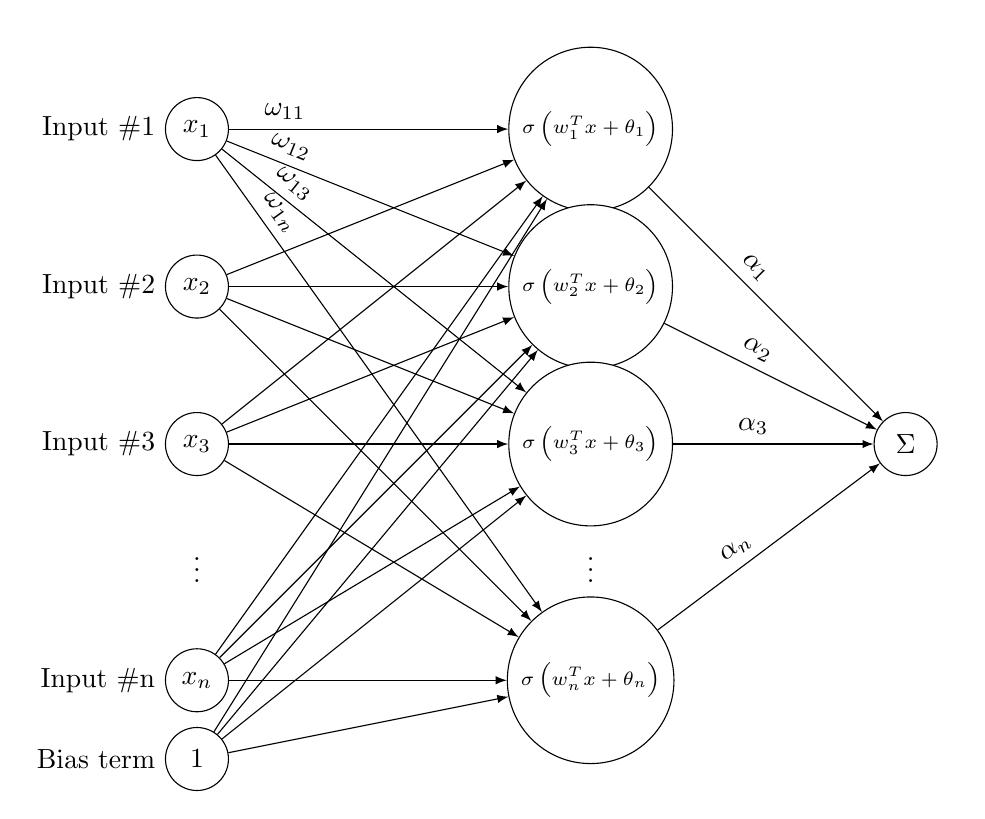
\begin{tikzpicture}
[   cnode/.style={draw=black,draw=black,fill=#1,minimum width=8mm,circle},
]
\tikzset{normal arrow/.style={draw,-latex}}
\node[cnode=white,label=0:] (s) at (9,-6) {$\Sigma$};
\node at (0,-7.5) {$\vdots$};
\node at (0,-10) {$\vdots$};
\node[cnode=white,label=180:Bias term] (x-5) at (0,-10) {1};
\node at (5,-7.5) {$\vdots$};
\foreach \x in {1,...,4}
{
	\pgfmathparse{\x<4 ? \x : "n"}	   
	\ifnum \x = 4
		\node[cnode=white,label=180:Input \#\pgfmathresult] (x-\x) at (0,{-2*\x-div(\x,4)}) {$x_{n}$};
		\node[cnode=white,label=90:] (p-\x) at (5,{-2*\x-div(\x,4)}) {\scriptsize$\sigma\left(w_n^Tx + \theta_n\right)$};

	\else

		\node[cnode=white,label=180:Input \#\pgfmathresult] (x-\x) at (0,{-2*\x-div(\x,4)}) {$x_{\x}$};
		\node[cnode=white,label=90:] (p-\x) at (5,{-2*\x-div(\x,4)}) {\scriptsize$\sigma\left(w_\x^Tx + \theta_\x\right)$};
	\fi
		\path[normal arrow] (p-\x) -- node[above,sloped,pos=0.4] {$\alpha_{\pgfmathresult}$} (s);
}
 

\foreach \x in {1,...,5}
{   
	\foreach \y in {1,...,4}
	{   
		\ifnum \x=1
			\ifnum \y=4
				\path[normal arrow] (x-\x) -- (p-\y) node[above,sloped,pos=0.15] {$\omega_{\x n}$};
			\else
				\path[normal arrow] (x-\x) -- (p-\y) node[above,sloped,pos=0.2] {$\omega_{\x\y}$};
			\fi
		\else
		\path[normal arrow] (x-\x) -- (p-\y); 
		
		\fi
		
		%\draw (x-\x) -- (p-\y) node[above,sloped,pos=0.3] {$\omega_{\x\y}$};
	}
}
\end{tikzpicture}

\end{center}


\begin{center}

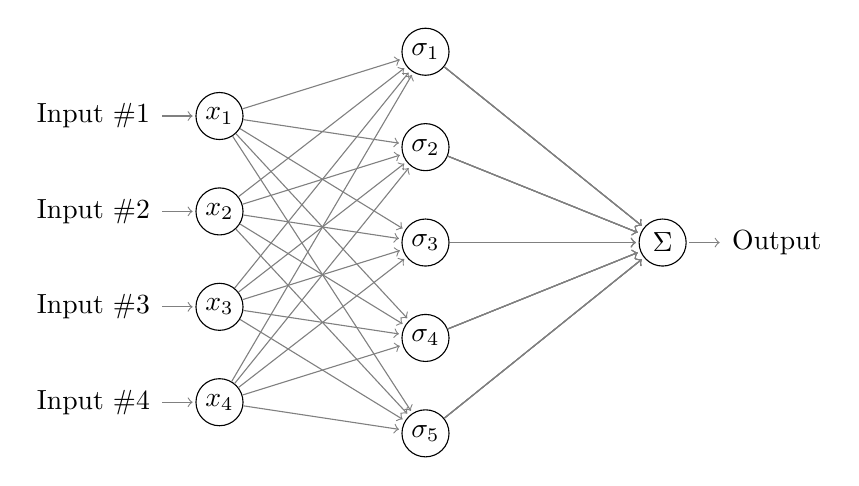
\begin{tikzpicture}[shorten >=1pt,->, draw=black!50, 
node distance = 6mm and 24mm,
start chain = going below,
every pin edge/.style = {<-,shorten <=1pt},
neuron/.style = {circle, draw=black, fill=#1, 
	minimum size=17pt, inner sep=0pt,
	on chain},
annot/.style = {text width=4em, align=center}
]
% Draw the input layer nodes
\foreach \i in {1,...,4}
\node[neuron=white!50,
pin=180:Input \#\i] (I-\i)    {$x_{\i}$};
% Draw the hidden layer nodes
\node[neuron=white!50,
above right=6mm and 24mm of I-1.center] (H-1)     {$\sigma_{1}$};
\foreach \i [count=\j from 1] in {2,...,5}
\node[neuron=white!50,
below=of H-\j]      (H-\i)    {$\sigma_{\i}$};
% Draw the output layer node
\node[neuron=white!50, pin= {[pin edge=->]0:Output}, right=of H-3]  (O-1)  {$\Sigma$};


% Connect input nodes with hidden nodes and 
%  hiden nodes with output nodes with the output layer
\foreach \i in {1,...,4}
\foreach \j in {1,...,5}
{
	\path (I-\i) edge (H-\j)
	(H-\j) edge (O-1);
}
\end{tikzpicture}
\end{center}


Neural networks with sigmoidal activation functions can approximate to arbitrary accuracy any functional continuous mapping from one finite-dimensional space to another, provided the number N of hidden units is sufficiently large.

		

wiki: "A sigmoid function is a mathematical function having a characteristic "S"-shaped curve or sigmoid curve. Often, sigmoid function refers to the special case of the logistic function defined by the formula"

$$
\sigma(x) = \frac{1}{1+e^{-x}}
$$



\begin{figure}[h]
	\centering
	\includegraphics[width=\linewidth]{sigmoid14_8}
	\caption{Sigmoid function, $\sigma(x) = \frac{1}{1+e^{-x}}$}
\end{figure}

\newpage

Let $I_n$ denote the n-dimensional unit cube, $[0,1]^n$. The space of continous functions on $I_n$ is denoted by $C(I_n)$ and we use $||f||$ to denote the supremum norm of an $f \in C(I_n)$. The space of finite, signed regular Borel measures on $I_n$ is denoted by $M(I_n)$.



\begin{definition}
	We say that $\sigma$ is sigmoidal if
	\begin{eqnarray*}
		\sigma(x) \rightarrow \begin{cases} 1 \;\;\;\text{as} &x \rightarrow +\infty\\ 0 \;\;\;\text{as} &x \rightarrow -\infty\end{cases}
	\end{eqnarray*}
	
\end{definition}

\begin{definition}
We say that $\sigma$ is discriminatory if for a measure $\mu \in M(I_n)$ 

$$
\int_{I_n} \sigma \left( y^Tx + \theta \right) d\mu(x) = 0
$$
for all $y\in \mathbf{R}$ and $\theta \in \mathbf{R}$ implies that $\mu = 0$.
	
\end{definition}


Hahn-Banach theorem shows how to extend linear functionals from subspaces to whole spaces. Moreover, we can do it in a way that respects the boundedness
properties of the given functional. The most general formulation of the theorem requires a preparation

\begin{definition}
A sublinear functional is a function $f:V \rightarrow \mathbf{R}$ on a vector space $V$ which satisfies subadditivity (1) and positive homogenity conditions (2)
\begin{eqnarray}
f\left(x+y\right) &\leq& f\left(x\right) + f\left(y\right) \;\;\;\;\;\;\;\;\;\;\;\forall x,y  \in V \\
f\left(\alpha x\right) &=&\alpha f\left(x\right) \;\;\;\;\;\;\;\;\;\;\;\;\;\;\;\;\;\;\;\;\; \forall \alpha\geq 0, x \in V
\end{eqnarray}
\end{definition}

\begin{theorem}[Hahn-Banach theorem for real vector spaces]
	If $p : V \rightarrow \mathbf{R}$ is a sublinear function, and $\psi : U \rightarrow \mathbf{R}$ is a linear functional on a linear subspace $U \subset V$, and satisfying $\psi(x) \leq p(x)$ $\forall x \in U$.
	Then there exists a linear extension $\Psi:V \rightarrow \mathbf{R}$ of $\psi$ to the whole space $V$, such that
	
	\begin{itemize}
		\item $\Psi(x) = \psi(x)$ $\forall x \in U$
		\item $\Psi(x) \leq p(x)$ $\forall x \in V$
	\end{itemize}
	
	Rudin 1991, Th 3.2
	
	%Let $V$ be a real vector space and $p : V \rightarrow \mathbf{R}$ a sublinear %functional on $V$. Let $\psi$ be a linear functional defined on a subspace $U %\subset V$, and satisfying $\psi(x) \leq p(x)$ $\forall u \in U$. Then there %exists a linear functional $\Psi:V \rightarrow \mathbf{R}$ such that
\end{theorem}

\begin{theorem}[Riesz representation theorem]
	Let $H$ be a Hilber space over $\mathbf{R}$, and $T$ a bounded linear functional on $H$. If $T$ is a bounded linear functional on a Hilbert space $H$ then there exist some $g \in H$ such that for every $f \in H$ we have (http://www.math.jhu.edu/~lindblad/632/riesz.pdf)
	$$
	T(f) = \langle f,g \rangle \;\;\;\;\;\; \forall f \in H
	$$
	
	Any bounded linear functional T on the space of compactly supported continuous functions on $X$ is the same as integration against a measure $\mu$. (http://mathworld.wolfram.com/RieszRepresentationTheorem.html)
	$$
	Tf = \int f d\mu
	$$
	
\end{theorem}

\begin{theorem}[]
	Let $\sigma$ be any continous discriminatory function. Then finite sums of the form
$$
G\left(x\right) = \sum_{j=1}^{N} \alpha_j \sigma\left(w_j^Tx + \theta_j\right)
$$

are dense in $C(I_n)$. In other words, given any $f \in C(I_n)$ and $\epsilon >0$, there is a sum, $G(x)$, of the above form, for whic

$$
|G(x) - f(x)| < \epsilon \;\;\;\;\;\;\;\; \forall x \in I_n
$$
\end{theorem}

\begin{proof}
Let $S \subset C(I_n)$ be the set of functions of the form $G(x)$. Clearly $S$ is a linear subspace of $C(I_n)$. We claim that the closure of $S$ is all of $C(I_n)$. 

Assume that closure of $S$ is not all of $C(I_n)$. Then the closure of $S$, say $R$, is a closed proper subspace of $C(I_n)$. By the Hahn-Banach theorem, there is a bounded linear functional on $C(I_n)$, call it L, with the property that $L \neq 0$ but $L(R) = L(S) = 0$.

By the Riesz Representation Theorem, this bounded linear functional, L, is of the form 

$$
L(h) = \int_{I_n} h(x)d\mu(x)
$$

for some $\mu \in M(I_n)$, for all $h \in C(I_n)$. In particular, since $\sigma(y^Tx + \theta)$ is in $R$ for all $y$ and $\theta$, we must have that

$$
\int_{I_n} \sigma \left(y^Tx + \theta \right) d\mu(x) = 0
$$

for all $y$ and $\theta$.

However, we assumed that $\sigma$ was discriminatory so that this condition implies that $\mu = 0$ contradicting our assumpition. Hence, the subspace $S$ must be dense in $C(I_n)$.

This demonstrates that sums of the form

$$
G(x) \sum_{j=1}^{N} \alpha_j \sigma\left(y_j^Tx + \theta_j\right)
$$

are dense in $C(I_n)$ providing that $\sigma$ is continous and discriminatory.

\end{proof}


\subsection{visual proof}



\end{document}
